%\documentclass[manuscript]{aastex}
%\documentclass[preprint]{aastex}
\documentclass[preprint2]{aastex}
%\documentclass{emulateapj}


\usepackage{url}
\usepackage{amsmath}
\usepackage{amssymb}
\usepackage{mathrsfs}
\usepackage{natbib}
\usepackage{color}
\usepackage{ulem} %% emph goes back to old meaning if you remove this. (Added for sout)
\citestyle{apj}
\usepackage{amsfonts}
\usepackage{float}
\usepackage{graphicx}
\usepackage{color} 
\usepackage{savesym}
\savesymbol{captionbox}
\usepackage{caption}
\usepackage{subcaption}
%\captionsetup[table]{labelsep=newline}

\def\lap{\hbox{${_{\displaystyle<}\atop^{\displaystyle\sim}}$}}

\def\draftmark {\special{!userdict begin
  /bop-hook{gsave 100 600 translate -45 rotate /Times-Roman findfont
  75 scalefont setfont 0 0 moveto 0.9 setgray (\today) show grestore}def
end}}


% Note environment
\newcommand{\note}[1]{[$\blacktriangleright$~\textbf{#1}~$\blacktriangleleft$]}
\newcommand{\shane}[1]{{\color{blue}[\textbf{shane:} #1]}}
\newcommand{\eric}[1]{{\color{cyan}[\textbf{eric:} #1]}}


%\lefthead{}
%\righthead{}
\bibliographystyle{apj}
\begin{document}

\draftmark

\title{Measuring accretion impact radii with optical and gravitational 
wave observations of compact binaries}

\author{Eric Addison}
\affil{Department of Physics, Utah State University, Logan,
Utah 84322}

\author{Katelyn Breivik}
\affil{Center for Interdisciplinary Exploration and Research in
   Astrophysics (CIERA) \& Department of Physics and Astronomy,
   Northwestern University, Evanston, IL 60208}

\author{Shane L.\ Larson}
\affil{Center for Interdisciplinary Exploration and Research in
   Astrophysics (CIERA) \& Department of Physics and Astronomy,
   Northwestern University, Evanston, IL 60208}
\affil{Department of Physics, Utah State University, Logan, Utah 84322}

%\received{}
%\accepted{}

\begin{abstract}
One of the primary astrophysical sources for space-based gravitational
wave observatories will be ultra-compact binary star systems in the
Milky Way.  Of the millions of such systems in the galaxy, several
thousand will be individually resolvable to a spaceborne gravitational
wave observatory.  For a large number of these systems,
multi-messenger observing campaigns with both gravitational wave and
electromagnetic telescopes will be possible.  The multi-messenger
characterization of compact binaries provides a useful synergy of
observing capabilities that can be exploited to recover detailed
information about the underlying astrophysical processes in the
binary.  This paper discusses how simultaneous photon and
gravitational wave observations of mass transferring binaries can be
used to characterize the accretion disks around the primary.  The
results suggest that for a large number of systems at a variety of
inclinations, accretion disk radii can be measured to a precision of better than $5\%$.
This is comparable to measurements using electromagnetic observations
of eclipsing systems, but is important because it will work for a much
wider range of binary inclination angles, including non-eclipsing 
systems.
	
\end{abstract}

\keywords{PICK SOME KEYWORDS}

% ---------------------------------------------------
\section{Introduction}\label{sec:Intro}

The interface between astrophysics and gravitational wave astronomy is
an important, emerging area of research as new methods of analyzing
and correlating gravitational data with traditional electromagnetic
data are found.  Of particular interest are ultra-compact binary stars
in the Milky Way galaxy.  Population estimates based on observed local
space densities \citep{HBW,TRC} as well as population synthesis
calculations \citep{Nelemans1,Nelemans2,StarTrack} suggest that all
told, the Milky Way may be populated by as many as $10^{7}$
ultra-compact binaries.  This population will be dominated by white
dwarf systems, with fewer numbers of systems where at least one
component is a neutron star or stellar mass black hole.

The ultra-compact binaries are characterized by strongly bound
components (often mass transferring, or having evolved to their current
state through significant periods of mass transfer) and short orbital
periods.  Binaries with orbital periods of $P_{orb} \sim 10^{5}$ s to
$P_{orb} \sim 1$ s should be easily observable in the gravitational
wave spectrum by any future space-based observatory.  The archetype of
such detectors has been the Laser Interferometer Space Antenna (LISA)
\citep{LPPA}; current design concepts include the European eLISA-NGO
\citep{elisa}, and the US SGO \citep{SGOlow,SGOmid,SGOhi} designs.

The sheer numbers of ultra-compact binary systems are expected to
produce a confusion-limited foreground of gravitational waves, which
will blanket the gravitational wave spectrum below $f \sim 3$ mHz.  An
example of the expected level of the confusion limit is shown in
Figure \ref{fig.wdNoise} \citep{HilsBender}, plotted against the
nominal sensitivity curves \citep{SCG} for missions with $5$ Gm and
$2$ Gm armlengths.  Strong sources of gravitational waves will rise up
above this confusion foreground and be observable by a space-based
gravitational wave observatory.

\begin{figure}[h]
\centering
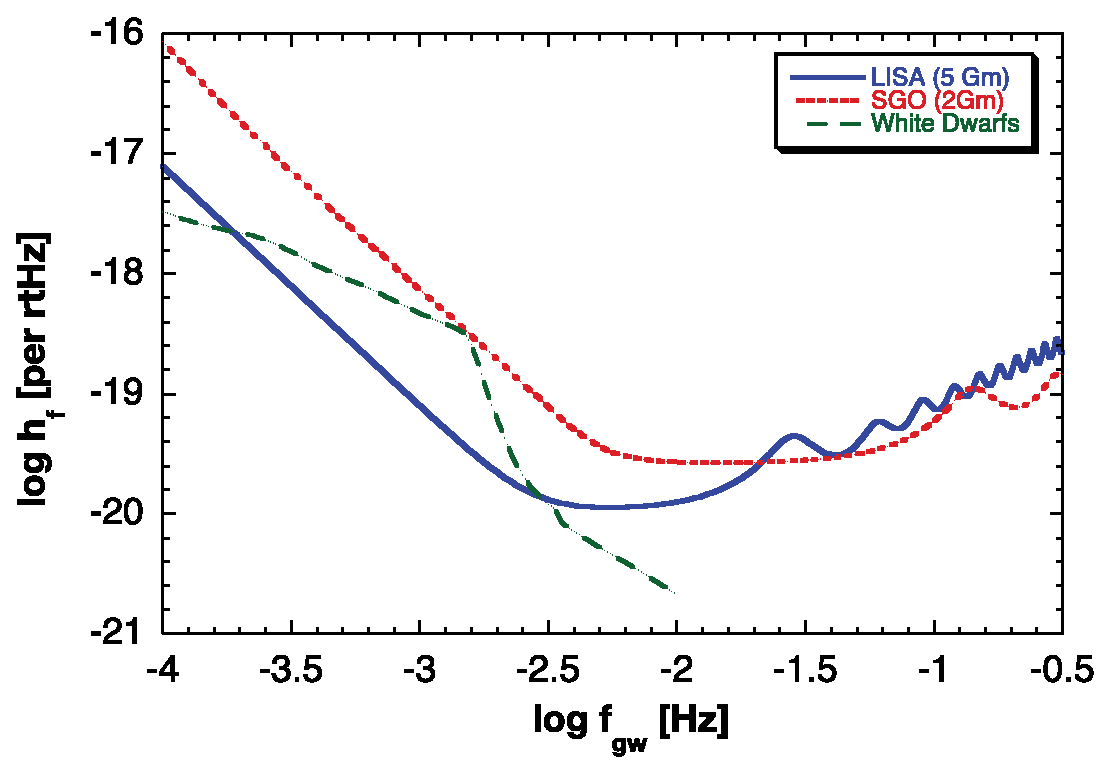
\includegraphics[width=80mm]{./figs/lisastandard.eps}
  \caption{The average gravitational wave power spectral amplitude,
  $h_{f}$, of the confusion foreground due to ultra-compact galactic
  binaries, plotted against the standard sensitivity curve \citep{SCG}
  for a 5 Gm (LISA) and 2 Gm (SGO) armlength observatory.  The assumed
  bandwidth is 1 year.}
  \label{fig.wdNoise}
\end{figure}

An interesting subset of the ultra-compact binaries are cataclysmic
variable stars (CVs), comprised of a primary white dwarf star and a
low mass secondary that has filled its Roche lobe and is transferring
mass to the primary; several thousand CVs have been cataloged in the
Milky Way (e.g., \cite{DownesCV}), but a gravitational wave detector 
in space will be sensitive to as many as 20,000 strewn throughout the 
galaxy.  The disparity in number here is the dim electromagnetic 
brightness of ultra-compact binary systems, which restricts EM 
detections to those that lie close to Earth, where as a gravitational 
wave detector will detect systems of this sort across the entire 
galaxy. Already, a growing number of ultra-compact
binaries and CVs have been observed and characterized with traditional
electromagnetic telescopes \citep{NelemansWiki}, a large fraction of
which are a class of helium cataclysmic variables (HeCV) similar to
the star AM {\it Canum Venaticorum} (AM CVn).  These systems have
primary white dwarfs with low mass helium companions providing mass
flow onto accretion disks of unknown radii.  They are expected to be 
strong gravitational wave radiators.

Realistic simulations on mock data \citep{MLDC1,MLDC2} have
shown that tens of thousands of these stars will be detectable by a
space-based gravitational wave detector as individually resolved
sources (e.g., \cite{CrowderCornish}), and several hundred of those
will be simultaneously detectable by electromagnetic telescopes, even
for mission designs more modest in scope than LISA
\citep{LLCN2013}.  A population of binaries that can be
observed with \textit{both} electromagnetic telescopes and
gravitational wave interferometers can be used as probes of the
fundamental astrophysics that governs these systems; this
multi-messenger mode of observations can reveal information that is
difficult or even impossible to extract otherwise.

Models of the accretion disks in HeCV systems have been studied in the
past, and suggest the disk radii will be around $75 \%$ of the primary
Roche radius \citep{Sulkanen81}, but this estimate is only certain to
within about $10 \%$.  Measurements of accretion disk radii in
ultra-compact binary systems have been made using eclipsing systems,
with results that are accurate to about $\sim 10\%$
\citep{1981ApJ...244..579S}.  Future space interferometry mission
concepts (\textit{e.g.}, \cite{SIM,TPF}) may make direct optical
imaging of close binary systems (like AM CVn) possible, allowing a
direct measurement of the accretion disk radius.  This letter
demonstrates how correlating optical observations of a mass
transferring CV system with simultaneous gravitational wave
observations by a space-based interferometer can yield a measure of
the primary accretion disk's radius.

The paper is organized as follows. Section \ref{sec.emGW} reviews the conceptual
model for the electromagnetic lightcurve and the gravitational wave
emission from these systems, as well as the
multi-messenger comparison.  Section \ref{sec.models} describes our
model for overflow and accretion, and our model for the light
curve from these systems.  Our results and discussion are presented in
Sections \ref{sec.demon} and \ref{sec.discussion}.

% =================================================================
\section{Multi-messenger signals}\label{sec.emGW}

\subsection{Electromagnetic lightcurve}\label{sub.emCurve}
Roche lobe overflow through the Lagrange point in ultra-compact
binaries will often lead to the formation of an accretion disk around
the primary star in mass transferring systems
\citep{LubowShu1975,Paczynski1977}.  A model \citep{Warner1995} that
can explain the optical properties of mass-transferring {HeCVs} has
a massive ($\sim 1 \rm{M}_{\odot}$) CO white dwarf embedded in an
accretion disk as a primary, and a less massive ($\sim 0.02
\rm{M}_{\odot}$) helium dwarf that has expanded to fill its
Roche lobe.  Material spills through the inner Lagrange point,
streaming onto the accretion disk and causing a bright hot-spot (see
Figure \ref{fig.overflow}).  This hot spot radiates approximately
radially outward from the disk; as the binary orbits, the spot
alternately turns towards and away from distant observers, modulating
the lightcurve.  This model has been applied to AM CVn {\it in
extenso} \citep{FFW,PHR,PHS} and successfully describes a variety of
signals present in the photometric lightcurve of this star.
Photometric observations have measured an orbital period of $\tau_{o}
= 1028.7325 \pm 0.0004$ s \citep{1998ApJ...493L.105H}, confirming previous
theoretical predictions \citep{PHS}.

\begin{figure}[t!]
  \centering
  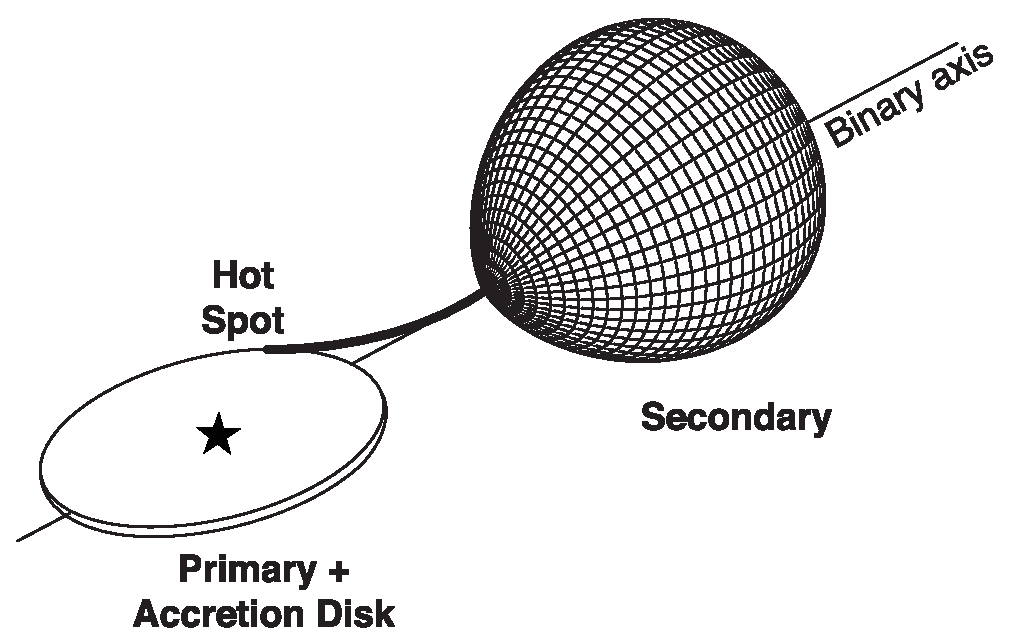
\includegraphics[width=80mm]{./figs/binaryModel.eps} 
  \caption{{\small The secondary companion has expanded to fill its 
  Roche lobe, which overflows, forming an accretion disk around the 
  white dwarf primary.  The point of accretion impact on the edge of 
  the disk creates a electromagnetically bright hot spot.}}
  \label{fig.overflow}
\end{figure}

Electromagnetic observation methods exist for determining accretion
disk radii from the lightcurve in \textit{eclipsing} binary systems
\citep{Ritter1980,Sulkanen81}.  In eclipsing systems, the accretion
disk can be occulted by the secondary, and then can itself occult the
secondary a half period later.  The contact points of the eclipse in
the electromagnetic lightcurve encode the exact position of the
binary components, and provide solutions for all the geometric
parameters of the binary, including the size of the accretion disk.
The error expected from these eclipsing methods is $\sim 10\%$,
estimated by \citet{1981ApJ...244..579S}.

% ---------------------------------------------------
\subsection{The gravitational wave signal}\label{sub.gwSignals}
The ultra-compact binaries are strong gravitational wave radiators in
the millihertz gravitational wave band.  In this regime, with orbital
periods on the order of several thousand seconds to tens of seconds,
the gravitational wave emission is well described by the quadrupole
formula \citep{PM,PM63}.  The gravitational wave emission extracts
energy and angular momentum from the binary on long timescales, until
ultimately the components merge (for compact stellar remnants like
neutron stars and black holes, the merger occurs at high frequencies,
in the regime covered by ground-based gravitational wave detectors
like LIGO \citep{ligoStatus2010}).  A particularly useful formulation
of the emission from compact binaries utilizing the quadrupole
formula is due to \citep{WahlquistBinary}, expressed in terms of
standard binary observational parameters (inclination, argument of
periapsis, longitude of the ascending node, etc.).  The overall
strength of the gravitational waves depends on a scaling factor
$h_{o}$:
\begin{equation}
	h_{o} = \frac{4G^{2}m_{1}m_{2}}{c^{4}a(1 - e^{2})D} =
	\frac{4G^{5/3}}{c^{4}(1-e^{2})}\frac{{\cal M}}{D}\left(2
	\pi f_{o} {\cal M}\right)^{2/3}
    \label{eqn.scalingAmplitude}
\end{equation}
where Kepler's third law has been used to express $a$ in terms of the
orbital frequency $f_{o}$, $D$ is the luminosity distance, and ${\cal
M} = (m_{1}m_{2})^{3/5}/(m_{1} + m_{2})^{1/5}$ is the ``chirp mass''
of the system.  It is expected that compact interacting binaries will
have become circularized through mass transfer and common envelope
evolution; gravitational wave emission also tends to circularize
binaries.  For circular binaries, $e = 0$, and the gravitational wave
frequency $f$ is simply related to the orbital frequency by $f = 2
f_{o}$.  Then the scaling amplitude is simply
\begin{equation}
	h_{o} = \frac{4G^{5/3}}{c^{4}}\frac{{\cal M}}{D}\left(
	\pi f {\cal M}\right)^{2/3} \ .
    \label{eqn.scalingAmplitude2}
\end{equation}
Gravitational wave detectors will detect two polarization states, the 
strength of which are expressed in terms of the scaling amplitude 
$h_{o}$. Using the quadrupole formula for an arbitrarily oriented 
circular binary gives \citep{1987GReGr..19.1101W}:
\begin{eqnarray}
   h_{+}(\theta) &=& h_{o}(\cos(2\phi)A_0 - \sin(2\phi)B_0 ) 
   \nonumber \\
   h_{\times}(\theta) &=& h_{o}( \sin(2\phi)A_0 +\cos(2\phi)B_0 ) \ .
   \label{eqn.wahlquistPolarization}
\end{eqnarray}
Here, $\phi$ can be interpreted as either the binary longitude of the
ascending node, or the gravitational wave polarization angle, and
\begin{align}
   A_0 &= -\dfrac{1}{2}[a+\cos^2(\iota)]\cos 2(\theta-\theta_n)\\
   B_0 &= -\cos(\iota)\sin 2(\theta-\theta_n)
\end{align}
are orientation dependent functions (additional terms for $e \neq 0$,
not treated in this work, may be found in
\citet{1987GReGr..19.1101W}).  The angle $\theta$ is the angular
position in the orbit (the ``true anomaly''), and $\theta_n$ is the
value of $\theta$ at the line of nodes, which we will set to zero for
convenience.  In a circular binary, the orbital phase angle
$\theta(t)$ is related to the gravitational phase angle $\varphi(t)$
by $\varphi(t) = 2\theta(t)$, where $\varphi(t)$ is the phase function
of the gravitational wave determined from the orbital dynamics and
evolution.  The gravitational wave phase for most of the population of
ultra-compact binaries is a simple function of the gravitational wave
frequency
\begin{equation}
    \varphi(t) = f t + \frac{1}{2}{\dot f} t^{2} + \phi_{0}\ ,
	\label{eqn.chirp}
\end{equation}
where $f$ and $\phi_{0}$ are the gravitational wave frequency and
wave phase at $t = 0$, and ${\dot f}$ is the \textit{chirp}.  The
gravitational wave contribution to the chirp, from the quadrupole
approximation, is
\begin{equation}
	{\dot f} =
	\frac{96}{5}\pi^{8/3}\frac{G^{5/3}}{c^{5}}f_{0}^{11/3}{\cal
	M}^{5/3}\ .
    \label{eqn.gwChirp}
\end{equation}

Astrophysical effects (such as spin orbit interactions \citep{Hut1981},
tidal interactions \citep{wvk2008} or mass transfer
\citep{DeloyeTaam2006}) will alter the angular momentum in the binary,
and thus the orbital period and observed frequency $f_{0}$.  The
ultimate effect is that there are many competing processes that drive
the evolution of angular momentum in the system.  It is clear that the
relative contributions of each physical process will alter the
interpretation of the orbital evolution derived from LISA's
gravitational wave observations, a matter that will be considered in a
future paper.

A LISA-like detector will have a frequency resolution related to the
mission duration $T_{obs}$ given by $\Delta f = 1/T_{obs}$; this is
the frequency ``bin width'' for observations.  As $T_{obs}$ lengthens,
the bin width narrows.  In general, a conservative estimate is that a
detector will detect a binary chirping if the frequency evolves by a
bin or more during the observing time, or ${\dot f} \gtrsim \Delta
f/T_{obs}$.  For the known parameters of AM CVn, Eq.\
\ref{eqn.gwChirp} predicts an evolution of ${\dot f} = 4.79 \times
10^{-19}$ Hz/s.  For a $T_{obs} = 1$ year observation, the limiting
chirp would be ${\dot f} = 1$ bin/yr $= 1.00 \times 10^{-15}$ Hz/s; AM
CVn's chirp falls well below this conservative threshold.  For the
purposes of this work, it is assumed that the binaries are all
monochromatic (non-chirping).

A spaceborne interferometer will characterize both {polarization} amplitudes as part
of its deconstruction of the data stream; the ratio of $h_{+}$ to
$h_{\times}$ is a direct measure of the inclination angle $\iota$ of
the binary, as shown in Figure \ref{fig.inclination}.  Knowledge of
the inclination angle provides further constraints on the model of the
electromagnetic lightcurve, making any derived radius of the
accretion disk more secure.
        
\begin{figure}[t!]
  \centering
  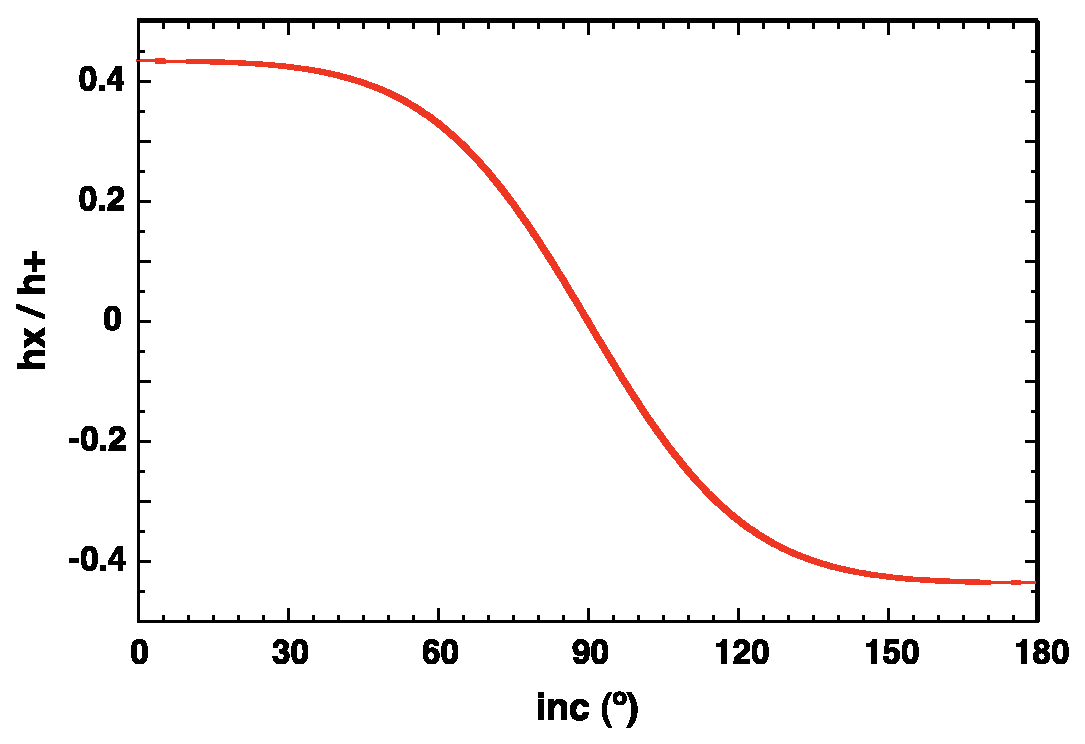
\includegraphics[width=70mm]{./figs/gwInclination.eps} 
  \caption{{\small Measuring the ratio of measured gravitational wave 
  polarization amplitudes, $h_{\times}/h_{+}$, is a measure of 
  the binary inclination angle, $\iota$.}}
  \label{fig.inclination}
\end{figure}



% -----------------------------------------------------------------
\subsection{Multi-messenger phase comparison}\label{sub.emGWphase}
The multi-messenger comparison being examined in this paper is
exploiting the periodic structure in both the gravitational wave and
the electromagnetic signals as a probe of the geometry of the source.
Consider a circularized ultra-compact binary with orbital frequency
$f_{o}$.  The gravitational wave frequency, $f$, is twice the orbital
frequency of the binary, $f = 2 f_{o}$.  In this case, the
gravitational wave signals peak at the times when the distance between the components of
the binary when projected onto the sky plane is minimized, which occurs when one of the components is at its closest distance to the observer. This provides a fundamental marker for the
orientation of the binary components in time.  By contrast, the
electromagnetic lightcurve shows variation (on orbital timescales)
corresponding to the underlying components of the binary changing
position and orientation with respect to the line of sight.  The tool
for determining the location of those structures, by measuring them
against the reference provided by the gravitational waves, is the
measured phase difference between the arriving gravitational waves and
the electromagnetic lightcurve.

The phase difference between the lightcurve and the gravitational 
waves at any observation time $t$ is
\begin{equation}
    \Phi(t) = \phi_{gw}(t) - \phi_{em}(t) = 2\pi t(f_{gw}-f_{em}) + 
    \alpha \ ,
    \label{eqn.phaseDifference}
\end{equation}
where $\alpha$ is a phase offset between the gravitational waves as
compared to the electromagnetic lightcurve at the time of
measurement.  The term $\alpha$ can encode a variety of physical and
geometric effects, but in principle can be divided into two basic 
flavors: effects that delay propagation after the signals are 
emitted, and model dependent delays that produce phase offsets when 
the signals are originally generated in the system.

For propagation delays, there are two fundamental origins.  First,
gravitational waves and photons could propagate at intrinsically
different speeds.  General relativity predicts that gravitational
waves should propagate at $v_{gw} = v_{em} = c$, but as a matter of
observational science this can be tested using multi-messenger
observations like those described here \citep{hazbounLarson2013}.  As
the expectations are for general relativity's predictions to be
correct, this paper assumes gravitational waves will propagate at the
speed of light: $v_{gw} = c$.  A second fundamental delay during
propagation could be experienced by the photons, traveling through
media with non-unit index of refraction: first through the
interstellar medium, and then through the Earth's atmosphere.  Given
the typical distance to sources that will be simultaneously detectable
in both EM and GW spectra, the typical phase delay from propagation
delays is estimated to be $\alpha_{prop} \sim 5 \times 10^{-11}$,
about 4 orders of magnitude less than the expected accuracy of the raw
phase measurements themselves \citep{gravitonSLL}, and can be safely
neglected for this analysis.

For geometric and model dependent phase differences, one must consider
the structure of the waves being observed.  The gravitational wave
structure is simple.  The ultra-compact binaries being considered here
are assumed to be circular and monochromatic, with the waveforms being
accurately described by the quadrupole radiation formula.  In this
context, the gravitational waves are sinusoidal.  Even for systems
that harbor small amounts of eccentricity, the signals will still be
exceedingly clean (both cases are shown in Figure
\ref{fig.gwSignals}).  The peaks in the gravitational wave signals
correspond to times when the binary components reach their closest distance to the observer; thus, the gravitational waves
provide an absolute reference for locating the binary axis orientation
as a function of time.  There is an ambiguity associated with the
quadrupolar nature of the gravitational radiation pattern --- it peaks
when one component is at its closest distance to the observer, but also $180^{\circ}$ away in the orbit, when
the positions of the binary components are reversed (this is most
obviously indicated in the gravitational wave frequency, which is
twice the orbital frequency, $\omega_{g} = 2 \omega_{orb}$).

\begin{figure}[t!]
  \centering
  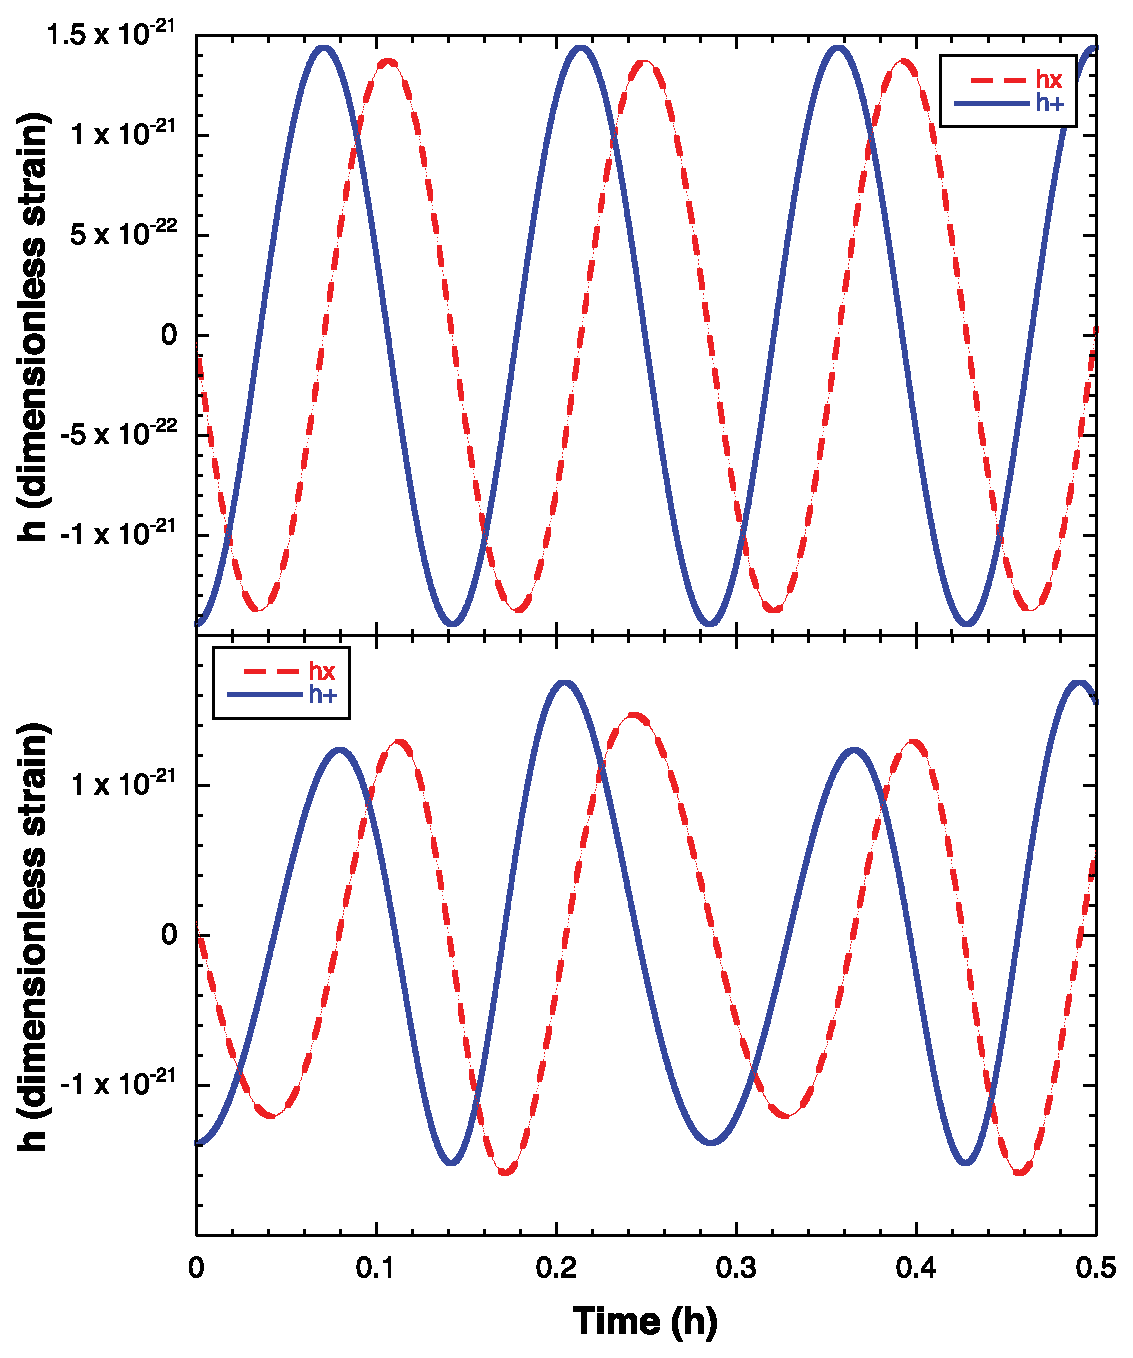
\includegraphics[width=80mm]{./figs/plotAMCVn.eps} 
  \caption{{\small Simulated gravitational wave signals for AM CVn 
  using current, best known parameters \cite{NelemansWiki}.  Top 
  panel shows the signal for a purely circular, monochromatic system. 
  Lower panel illustrates how signal changes if system had moderate 
  eccentricity ($e = 0.1$), but otherwise identical parameters.}}
  \label{fig.gwSignals}
\end{figure}

By contrast, the electromagnetic lightcurve is rich in structure, 
with shapes and peaks in the curve being the result of the changing 
aspect of the system's internal components during the course of an 
orbit. There are several primary contributions to the lightcurve 
shape: emission from the white dwarf primary; emission from the Roche 
expanded secondary giving ellipsoidal variations as the secondary 
shape rotates relative to the line of sight; emission from the 
accretion disk; and lastly, emission from the hot spot where the 
overflow stream impacts the accretion disk. Consequently one must choose where we want the gravitational wave signal and the lightcurve signal to line up, and the offset from this alignment point to the point of zero binary phase constitutes the geometrical part of $\alpha$.

In this paper we are interested in characterizing the accretion disk radius
by measuring the phase of the hot spot compared to the phase of the
gravitational wave signal. In this context then, the value of the
parameter $\alpha$ in Eq. \ref{eqn.phaseDifference} is affected by the geometric angle $\alpha_{\star}$ illustrated in Figure
\ref{fig.overflowAlpha}, the angle between the binary axis and the
impact point on the accretion disk. For a given model of the overflow
stream, the measured value of $\alpha_{\star}$ will correspond to a unique
accretion disk radius.  The ability to measure $\alpha_{\star}$ will be
limited by the errors associated with each of the independent phase
measurements, and by our ability to recognize the contribution of the
hot spot to the electromagnetic lightcurve.

\begin{figure}[t!]
  \centering
  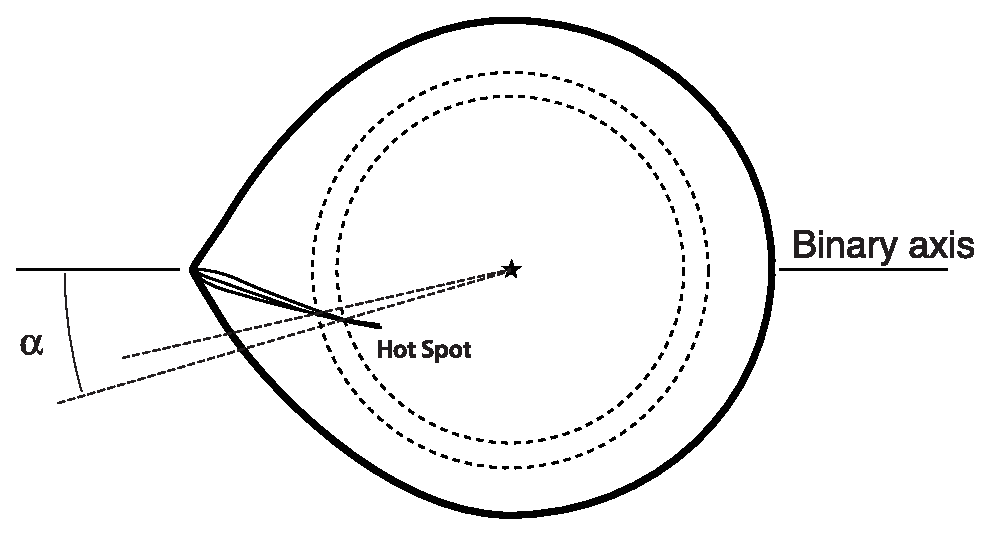
\includegraphics[width=80mm]{./figs/Overflow2.eps} 
  \caption{{\small The overflow stream from the donor
  creates a hot spot at the impact point on the accretion disk.  The
  value of the angle $\alpha_\star$ depends on the radius of the accretion
  disk.}}
  \label{fig.overflowAlpha}
\end{figure}


% =================================================================
\section{A simple model for ultra-compact mass overflow
binaries}\label{sec.models}


\begin{table*}[t!]
\caption{AM CVn Simulation Parameters}
\centering
\begin{tabular}{l l l l}
\hline \hline
Parameter & Notation & Value & Reference\\
\hline
Mass 1 & $m_1$ & $0.68M_{\odot}$ & 1\\
Mass 2 & $m_2$ & $0.125M_{\odot}$ & 1\\
Orbital Period & $P_{orb}$ & 1028.73 s & 2\\
Inclination & $\iota$ & $43^{\circ}$ & 1\\
Luminosity Distance & $d$ & 606 pc & 1\\
Disc Radius & $R_\text{disc}$ & $0.48a$ & 3\\
\hline
Char. Disc Temp. & $T_\text{disc}$ & 90000 K & Fit\\
Pole Temp. & $T_{\text{pole}}$ &  15065 K & Fit, 4\\
WD Temp. & $T_{WD}$ & 19473 K & Fit\\
Max HS Temp. & $T_{\text{HS}}$ & 131000 K & Fit\\
HS Cooling Parameter & $\zeta$ & 2.9828 & Fit\\
\hline
\multicolumn{4}{l}{\textbf{Notes.} Parameters below the horizontal line are fitted using our lightcurve model.}\\
\multicolumn{4}{l}{\textbf{References.} (1) \citealt{2006MNRAS.371.1231R}; (2) \citealt{1998ApJ...493L.105H};}\\ 
\multicolumn{4}{l}{(3) \citealt{1998A&A...332..939S}; (4) \citealt{2006MNRAS.371.1231R}.}
\end{tabular}
\label{table.params}
\end{table*}

\subsection{Model System: AM CVn} \label{sec.modelParameters}
Many ultra-compact binaries have already been identified as candidate
\textit{verification binaries} for space-based gravitational wave
detectors \citep{NelemansWiki}.  For the purposes of demonstration,
this paper uses as canonical parameters the current known values for
\textit{AM Canum Venaticorum} (AM CVn), the archetype for a large
number of ultra-compact binaries that are expected to be
visible in gravitational waves.  The physical parameters for AM CVn
are: $m_{1} = 0.68M_{\odot}$, $m_{2} = 0.125M_{\odot}$, and $\omega =
6.108 \times 10^{-3}$ s$^{-1}$ (a circular binary with semi-major axis
$0.21 R_{\odot}$). The disc radius is estimated to be $R_d
= 0.478a$ \citep{1998A&A...332..939S}    
%\note{eric: the following sentence was taken from the old section 4 subsection called ``output''; all discussion of our model for the system goes here, but this sentence about temp parameters and fitting techniques doesn't make sense to me at the moment; it needs clarified to explain what you were fitting, and how that leads to the table (which was also moved here)} 
The temperature parameters were estimated by minimizing the $L_2$ error between the output of our lightcurve model (see section \ref{sec.LightCurve}) and the observed lightcurve. A temperature $T=10^{4}K$ is adopted as an initial guess for the pole
temperature of the secondary \citep{2006MNRAS.371.1231R}. 



% -----------------------------------------------------
\subsection{Overflow simulations}\label{sec.Overflow}
\subsubsection{Equations of Motion}
In order to demonstrate this method for measuring the
accretion disk radius, a simple model of the accretion overflow was
created using the restricted three body approximation
\citep{Flannery1975}.  In the co-rotating frame of the binary, the
accelerations on a fluid particle in the $x$ and $y$ directions may be
written as
\begin{align}
	{\ddot x} & = -\frac{G m_{1}}{r_{1}^{3}}\left(x
	- \frac{aq}{1 + q}\right) - \frac{G
	m_{2}}{r_{2}^{3}}\left(x +
	\frac{a}{1 + q}\right) \nonumber \\
	& + \omega^{2}x + 2 \omega{\dot y} - \xi {\dot x}\ ,
	\label{eqn.xDDot}
\end{align}
and
\begin{align}
	{\ddot y} & = & -\frac{G m_{1}}{r_{1}^{3}}y - \frac{Gm_{2}}{r_{2}^{3}}y + \omega^{2}y - 2\omega{\dot x} - \xi {\dot y}\ , 
	\label{eqn.yDDot}
\end{align}
Here $\omega = 2\pi f_{orb}$ is the orbital angular velocity of the
stellar components, $q = m_2/m_1$ is the mass ratio, and $\xi$ is a
parameter that characterizes the viscous drag on the fluid element.


In simulation, the equation is non-dimensionalized by introducing
scaling factors $M$ (total mass) for mass, $a$ (binary separation) for
length, $\omega^{-1}$ for time, and $GM/a$ for potential.  The
dimensionless equations then read
\begin{eqnarray}
   \tilde{x}'' &=& -\dfrac{\mu}{\tilde{r}_1^3}(\tilde{x} - \tilde{a}Q) -
   \dfrac{(1-\mu)}{\tilde{r}_2^3}\left (\tilde{x} +
   \dfrac{\tilde{a}}{q}Q\right ) \nonumber \\
   & &\quad + \tilde{x} + 2\tilde{y}' - \tilde{\xi}\tilde{x}' 
   \nonumber \\
   \tilde{y}'' &=& -\dfrac{\mu}{\tilde{r}_1^3}\tilde{y} -
   \dfrac{(1-\mu)}{\tilde{r}_2^3}\tilde{y} + \tilde{y} - 2\tilde{x}' -
   \tilde{\xi}\tilde{y}'\ ,
   \label{eqn.dimensionlessSystem}
\end{eqnarray}
where $\tilde{x}$ and $\tilde{y}$ are dimensionless coordinates,
$\tilde{\xi}$ is the dimensionless viscosity coefficient, $\mu$ is the
mass fraction $\mu = m_1/M$, $Q=q/(1+q)$, and prime denotes
differentiation with respect to the dimensionless time variable.

These equations are simultaneously numerically integrated to give 
the position and velocity of particles in the overflowing accretion 
stream. The geometric information regarding the position of the 
stream is an essential player in the determination of the accretion 
disk radius, and the stream particle velocity at disk impact is used 
in the energetic calculations that give the model brightness for the 
hot spot.

From this point on, tildes will be dropped and quantities discussed in
the context of the overflow simulation will be the dimensionless
variables.

% -------------------------------------------------------------
\subsubsection{Stream Coherence}
Early numerical simulations \citep{Flannery1975} of matter overflow in
cataclysmic variables suggested the stream maintains coherence as it
falls toward impact.  Coherence in the overflow stream through impact
with the primary accretion disk is a necessity to understanding the
variable lightcurve created by cataclysmic variable stars such as AM
CVn.  To evaluate the stream coherence in this model, initial 
velocity data for Eq.\ \ref{eqn.dimensionlessSystem} were drawn from the
Maxwell-Boltzmann Speed Distribution:
\begin{equation}
   f(\upsilon)=\frac{\sqrt{\frac{2}{\pi}}\upsilon^2
   \exp(\frac{-\upsilon^2}{2\eta^2})}{\eta^3}
\end{equation}
where $\eta$ is determined by the thermal coefficient:
\begin{equation}
	\eta=\sqrt{\frac{kT}{m}}
\end{equation}
and $k$, $T$ and $m$ are Boltzmann's constant, the temperature of the
secondary, and the mass of the particle in the stream. The velocities were constrained by angle $\theta=\pm57^{\circ}$, the
maximum opening angle of the gravitational equipotential that passes
through the inner Lagrange point.  

%\textcolor{red}{\note{Shane: I don't understand this ``extreme" business for velocity. I just drew randomly from the Boltzmann dist.}} The extreme initial velocities were
%then taken to be the most probable speed of the Maxwell-Boltzmann
%speed distribution with temperature $T$, giving
%\begin{equation}
%	\upsilon=\sqrt{\frac{2kT}{m}}
%\end{equation}
%and the extreme angles given by $\theta$.

Taking the canonical particle mass to be the mass of a proton, the
simulation was run $2,500$ times pulling randomly from the speed
distribution and attaching that speed to an angle drawn from a uniform
distribution in the range of $\theta$.  Results of this simulation are
shown in Figure \ref{fig.streamSim}, in the co-rotating frame of
the binary.  This histogram show the injected parameters, while the
trajectory plot shows overlays of all $2,500$ runs in the
equipotential space dominated by the white dwarf (the vertex of the
equipotential boundary drawn at $y = 0$ is the Lagrange point between
the primary and secondary).  All of the trajectories, irrespective of
initial conditions at the overflow point, coalesce around a central
trajectory.

\begin{figure*}
        \centering
        \begin{subfigure}[b]{0.45\textwidth}
	        \centering
                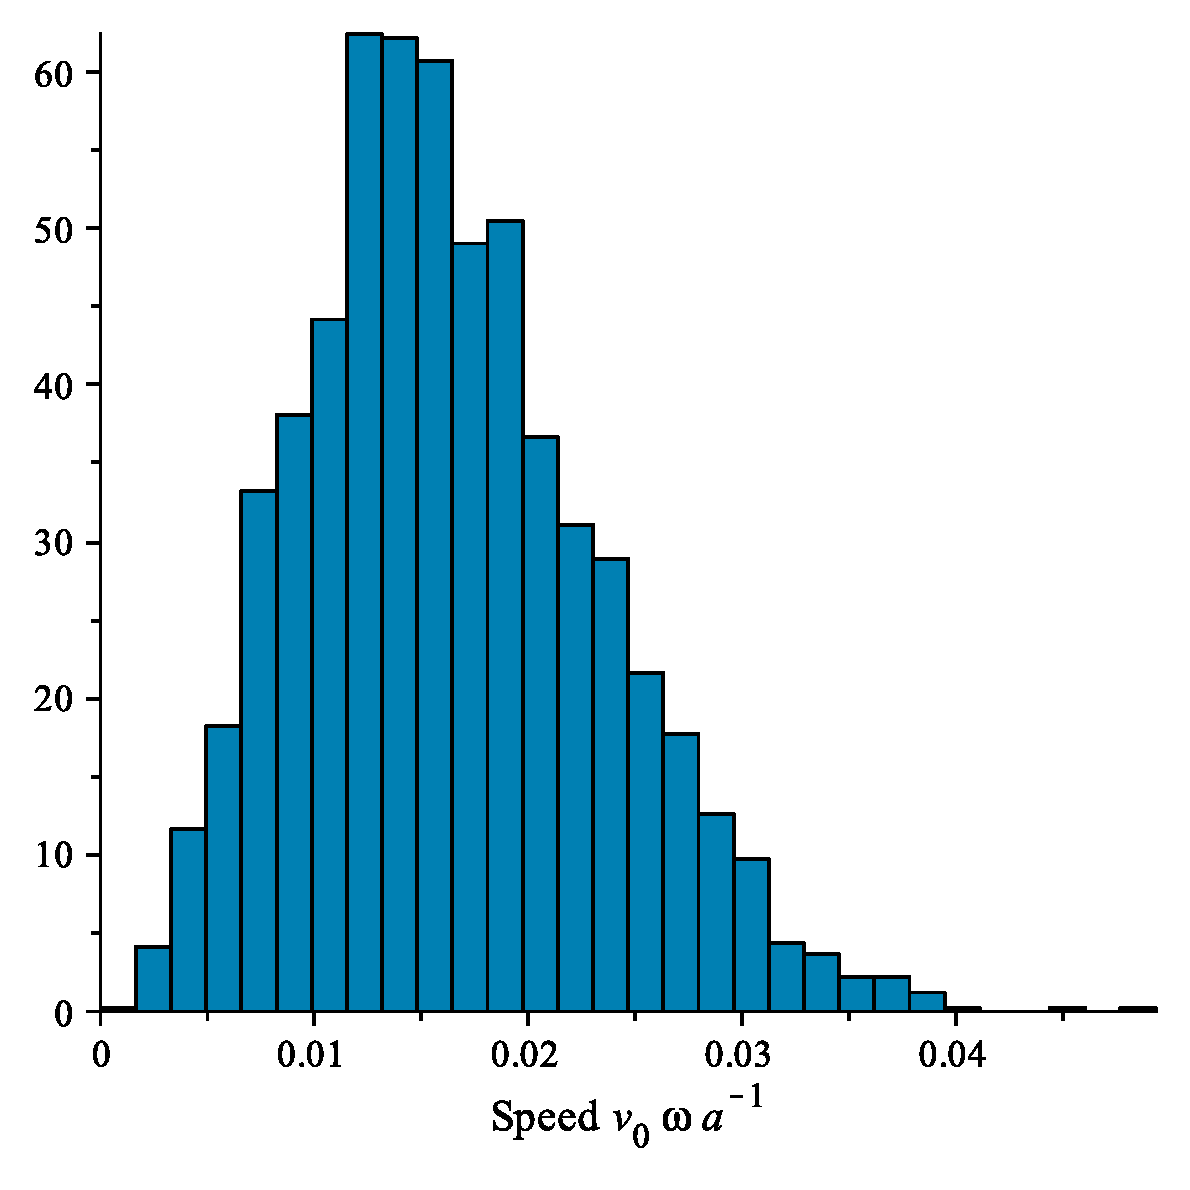
\includegraphics[width=\textwidth]{./figs/speed_hist}
                \caption{Histogram of sampled speeds with most probable speed $v_{p} = \sqrt{2}\eta = 0.0145$.}
                \label{fig.streamHist}
        \end{subfigure}%
        \quad %add desired spacing between images, e. g. ~, \quad, \qquad etc.
          %(or a blank line to force the subfigure onto a new line)
        \begin{subfigure}[b]{0.45\textwidth}
        			\centering
                \includegraphics[width=\textwidth]{./figs/Overflow2000}
                \caption{Overflow stream simulation for AM CVn parameters.  Stream
  is visually observed to maintain coherency until self-impact.}
                \label{fig.coherentStream}
        \end{subfigure}
        \caption{Overflow stream simulation figures.}
        \label{fig.streamSim}
\end{figure*}

% -------------------------------------------------------------
\subsubsection{Hot Spot Phase Angle}
Based on the stream coherence simulation, the trajectory of the matter
overflow stream is known until the time it intersects the accretion
disk.  The HS phase offset angle, $\alpha_\star$, is measured from the binary
axis (located from the gravitational waves) to the hot spot impact
point (measured from the electromagnetic lightcurve), and using the
trajectory model yields the accretion disk radius at which the
trajectory crosses the angle $\alpha_\star$ ({\it i.e.}, the radius of the
disk when it intersects the matter stream).  For the AM CVn
demonstration parameters, Figure \ref{fig.impact_angle} displays
calculated values of the HS phase offset angle $\alpha_\star$ for a range of
disc radii lying within the primary's Roche radius.  Larger disc radii
show a small spread in impact angles ($\sim 2^{\circ}$), a consequence
of tight stream coherency, while smaller radii result in a larger
impact spread (as high as $\sim 10^{\circ}$) due to the oblique angle
of attack at impact.

\begin{figure}[h]
  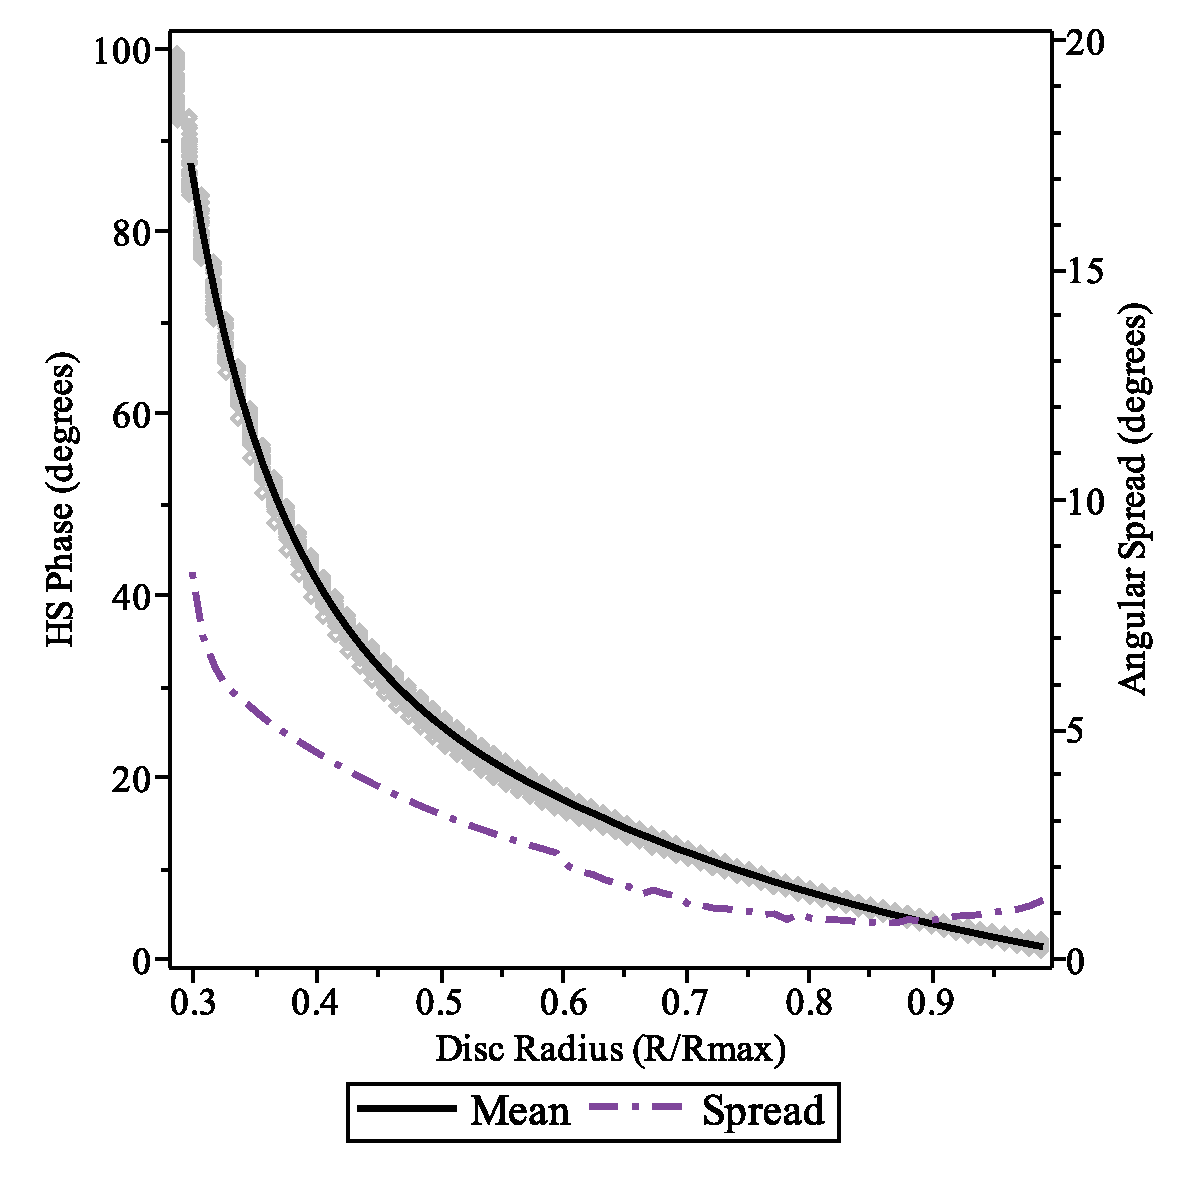
\includegraphics[width=\columnwidth]{./figs/impact_angle_0.06.eps}
  \caption{Stream impact angle $\alpha_\star$ for various disc radii,
  ranging up to the size of the primary Roche Lobe.  Radius values are
  scaled by the value $R_\text{max}$, which is defined as the distance
  from the primary to the $L1$ Lagrange point.  The grey envelope
  shows the spread of impact angles for a random selection of initial
  velocities, while the black line plots the mean of the spread.  The
  dashed line plots the angular spread of the stream impact with
  values on the right vertical axis.}
  \label{fig.impact_angle}
\end{figure}

% -------------------------------------------------------------
\subsubsection{Viscosity Term}
The overflow stream consists of a collection of infalling particles, which will
have some measure of interaction with each other, plausibly
influencing the trajectory.  To explore this, a dimensionless
viscosity parameter is used in the equations of motion, Eq.\
\ref{eqn.dimensionlessSystem}.  In general, this value is expected to
be small, $\xi \lesssim 0.1$, but even smaller values are typical in
modern accretion simulations \citep{2008A&A...487..671K}, to the point
of using inviscid flow \citep{1992MNRAS.255P..17S}.  By examining the
range of $\xi$ over which the stream crosses itself, it is seen that
neither the mean impact angle nor the angular spread vary
significantly in the range $0 \le \xi \le 0.3$ (see Figure
\ref{fig.impact_angle_various}).  For viscosity values larger than
$\xi \gtrsim 0.3$, these simulations enter the regime where the stream
will not cross itself, but rather it will impact the primary directly,
resulting in no disc formation.  This implies that the stream
viscosity does not significantly affect the angle $\alpha_\star$.  A value
of $\xi = 0.06$ is adopted for the simulations presented here.

\begin{figure*}[t!]
  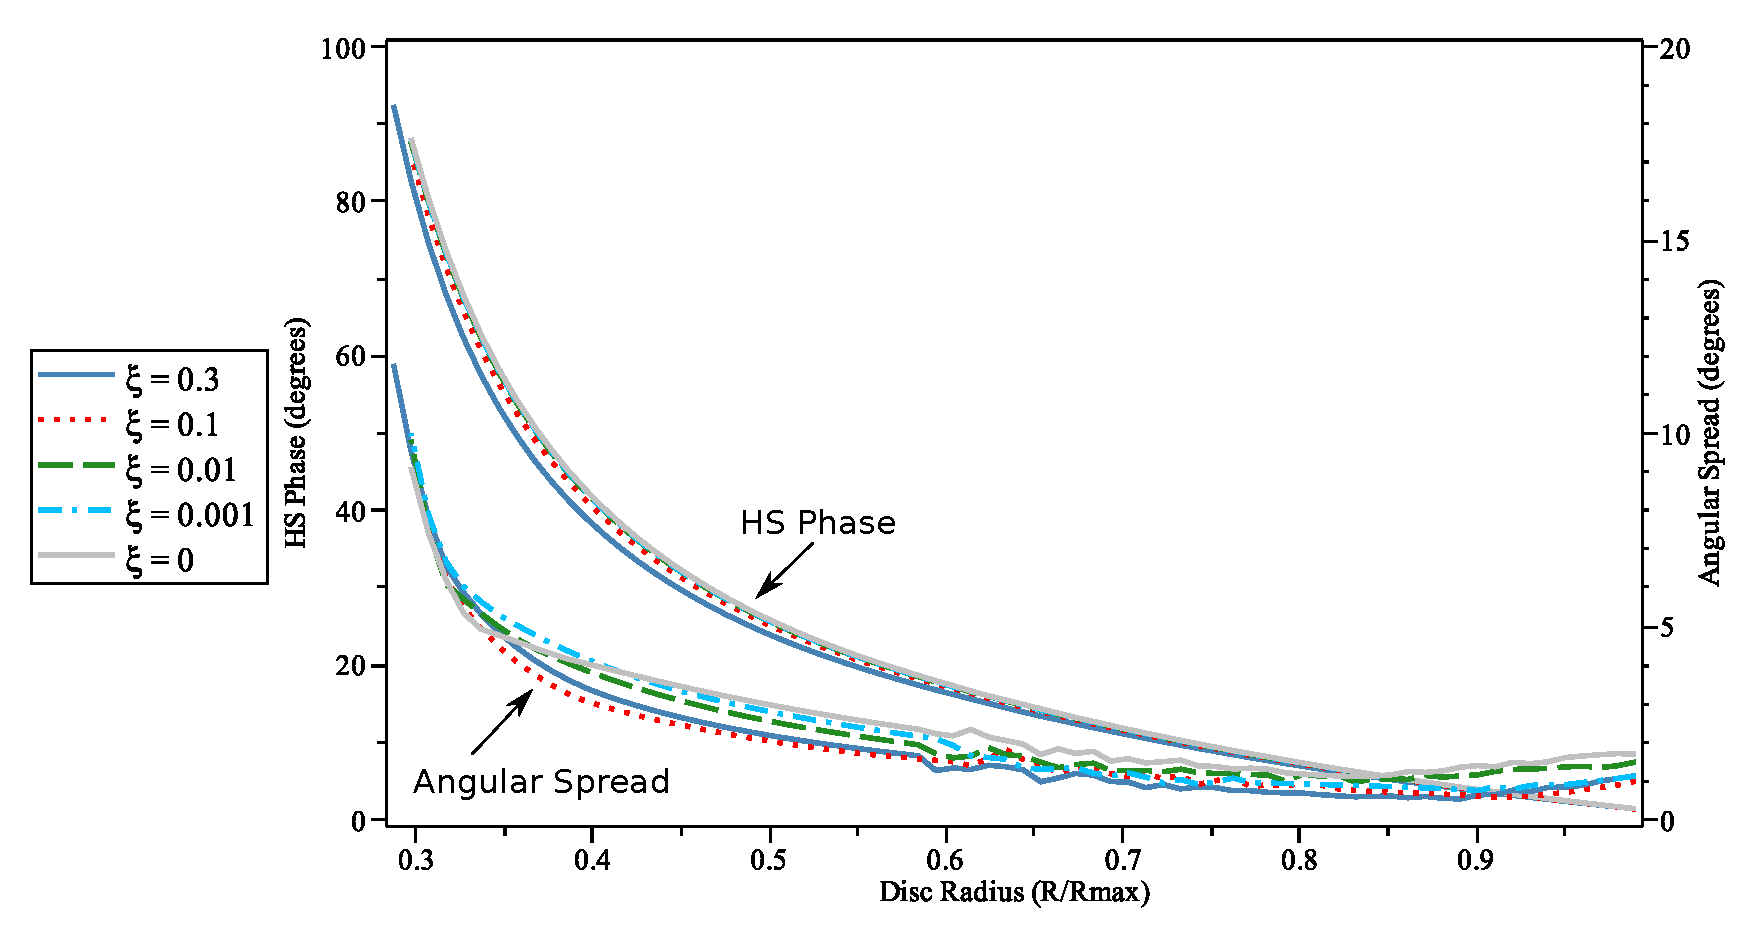
\includegraphics[width=\textwidth]{./figs/impact_angle_various2.eps}
  \caption{HS phase offset angle $\alpha_\star$ for various values of
  dimensionless viscosity $\xi$.  Note that the mean impact angle and
  angular spread are essentially unchanged over many orders of
  magnitude. }
  %\note{eric: here your fig caption says ``stream impact  angle'' but the vertical axis is ``HS phase'' -- pick one, and   adjust the other to be consistent.}
  \label{fig.impact_angle_various}
\end{figure*}


% -------------------------------------------------------------
\subsection{Lightcurve simulations}\label{sec.LightCurve}

Since simultaneous, coordinated electromagnetic and gravitational wave
observations of ultra-compact binaries do not exist (yet), simulated
lightcurve data are generated for this study.  Lightcurves are
generated via a simple geometric model with numerically modeled
accretion implemented in a \begin{sc}matlab\end{sc} program.  In this
simulation, a close binary system with an accretion disc and a hot
spot is rotated in three dimensions, and the observed portions of the
bodies in the system are used to generate a synthetic lightcurve.
This is a geometry based simulation; physical processes such as gravitational attraction are not
explicitly computed.  This is a well known basis for lightcurve simulations,
e.g. \cite{1971ApJ...166..605W}.

% -------------------------------------------------------------
\subsubsection{Setup}

There are four distinct objects in the simulation: the primary star,
the accretion disc, the hot spot, and the Roche lobe filled by the
secondary star.  Three dimensional point clouds are generated for each
object in appropriate orbital positions, which are then used to
compute the three dimensional \textit{convex hull} of each object.
The convex hull of a 3-D point cloud is a triangulation of the
bounding surface of the cloud, i.e. a set of vertex-connected
triangles such that all points in the cloud are either triangle
vertices or interior to the surface formed by the triangulation.  For
each triangle in the triangulation, the geometric center, area, and
normal vector are computed.  Temperature profiles (described in the
next section) are mapped onto the objects by assigning a temperature
for each triangle in the convex hulls, based on input parameters for
the simulation.  The simulation can be run for as long as desired to
generate lightcurves of arbitrary length.

% -------------------------------------------------------------
\subsubsection{Temperature Profiles}
Temperature values for the Roche Lobe are generated by the law of
gravity darkening, $T_e \propto g^{1/4}$
\citep{1967ZA.....65...89L,1924MNRAS..84..665V}. This leads directly
to an expression for the temperature at any point on the Roche Lobe given the pole temperature $T_{pole}$:
\begin{equation}
   \dfrac{T(x,y,z)}{T_{\text{pole}}} = \left
   [\dfrac{g(x,y,z)}{g_{\text{pole}}}\right ]^{1/4}
\end{equation}
where $T_{\text{pole}}$ and $g_{\text{pole}}$ are the values of
temperature and gravitational acceleration at the star pole.
$T_{\text{pole}}$ is generally taken to be the effective temperature
of a comparable field star \citep{1997ApJ...477..876O}, and
$g_{\text{pole}}$ can be found by taking the gradient of the known
gravitational potential at the pole of the Roche Lobe.

The temperature profile for the disc is a simple energy conservation
based model given by
\begin{equation}
   T = T_{\text{disc}}\left (\dfrac{R}{r} \right )^{3/4} \left (1 -
   \sqrt{R/r} \right )^{1/4}
\end{equation}
where
\begin{equation}
   T_{\text{disc}} = \left ( \dfrac{3Gm_1\dot{m}_{1}}{8\pi \sigma R^{3}}
   \right )^{1/4}
\end{equation}
is a characteristic temperature of the disc with $\dot{m}_{1}$ the mass
transfer rate, $R$ the radius of the primary, $r$ the radial distance out from the center of the disc, and $\sigma$ the
Stephan-Boltzmann constant.

The hot spot is modeled as a sphere with center located at the edge
of the accretion disc, and assigned an exponentially decaying
temperature profile according to
\begin{equation}
   T(\hat{x}) = (T_{\text{HS}} - T_d)\exp \left ( -\zeta \hat{x}\right )
   + T_d
\end{equation}
where $\hat{x}$ is a dimensionless coordinate that ranges from $0 \le
\hat{x} \le 2$, given by $\hat{x} = (s - s_{\text{CM}})/R_{\text{HS}}
+ 1$, $s$ is the radial distance of the center of the hot spot from
the primary, $s_{\text{CM}}$ is the center of the hot spot,
$R_{\text{HS}}$ is the radius of the hot spot, $T_{\text{HS}}$ is the
maximum temperature on the hot spot, $T_d$ is the outer disc
temperature, and $\zeta$ is the spatial cooling rate. 

The primary white dwarf temperature is set as a constant value over a
sphere.

\begin{figure}[t]
   \centering
   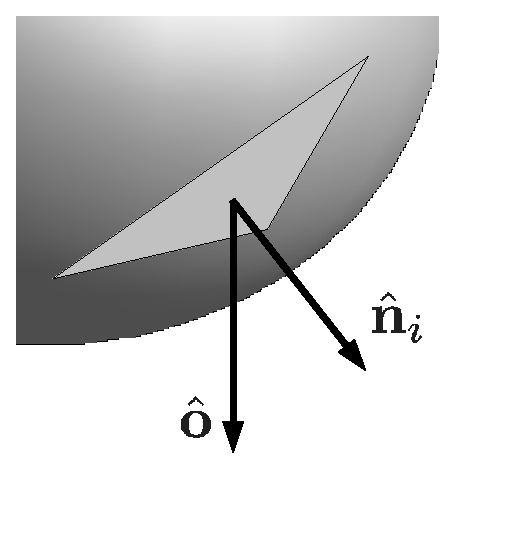
\includegraphics[scale=0.6]{./figs/vectors.eps}
   \caption{Illustration of observer vector and triangle normal 
   vector, overlaid on a convex hull element at the stellar surface.}
   \label{vecfig}
\end{figure}

% -------------------------------------------------------------
\subsubsection{Geometric Flux Projection}
\label{sec:geomFlux}
The lightcurve simulation assumes that the observer is positioned far away on the
negative $z$-axis, in which case the $xy$-plane is the sky plane for the observer.  At each time step, a point on the synthetic light
curve is computed as follows.  For the four objects in the simulation,
the normal vectors for each triangle in the convex hull triangulations
are examined to determine if the value of the $z$ component is
negative, i.e. has a component pointing toward the observer.
Triangles failing this condition are discarded for this iteration.
Next, the objects are ordered based on their $z$ coordinate,
essentially from lowest to highest.  The triangle centers of the first
object in the order are projected onto the $xy$-plane.  Subsequent
objects are also projected, however care is taken to avoid overlap of
the objects by use of a 2-D convex hull and a standard
point-in-polygon algorithm.  Triangles whose projected centers lie
interior to the convex hull of a previously projected object are
discarded, thus ignoring those triangles occulted by other objects in
the system.

The luminosity of each triangle visible to to the observer is
calculated using the Stefan-Boltzmann law. Total flux arriving at
Earth is then computed using the standard flux-luminosity
relationship, summed over $\mathcal{V}(t_k)$, the set of all visible
triangles at the $k$th time step:
\begin{equation}
   F(t_k) = \sum_{i \in \mathcal{V}(t_k)} \dfrac{\sigma A_i T_i^4
   (\hat{\textbf{o}} \cdot \hat{\textbf{n}}_i)}{4 \pi D_E^2}
\end{equation}
where $A_i$ and $T_i$ are the area and temperature of the $i$th
triangle, respectively, $\hat{\textbf{o}}$ is the unit vector
pointing toward the observer, $\hat{\textbf{n}}_i$ is the unit vector
normal to the $i$th triangle (see Figure \ref{vecfig}), and $D_E$ is
the distance to Earth.

This simulation calculates only raw bolometric blackbody
luminosities; more detailed effects such as frequency specific flux,
reflectance, etc. are not included. For the purpose of this paper,
however, these omissions are acceptable.  A lightcurve generated for 
the AM CVn model parameters is plotted against observed lightcurve 
data in Figure \ref{fig.LC_output}.

\begin{figure}[t]
  \centering
  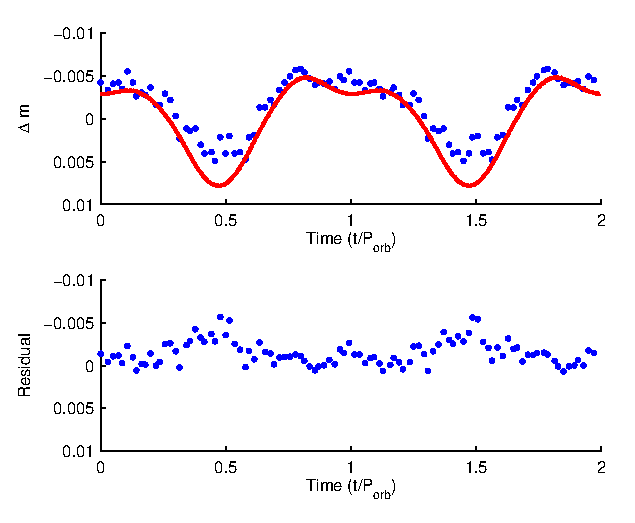
\includegraphics[width=\columnwidth]{./figs/amCvn_plus_residuals.eps}
  \caption{Simulated lightcurve for AM Canum Venaticorum in the top panel, displayed as
  magnitude deviation from mean, $\Delta m$. Solid line shows
  simulation output, dots represent actual AM CVn data
  \citep{1998ApJ...493L.105H}. Bottom panel shows residuals between model and observation.}
  \label{fig.LC_output}
\end{figure}



% -------------------------------------------------------------
\subsection{GW Phase Calibration}
\label{sec.GWcal}

\begin{figure*}[t]
\centering
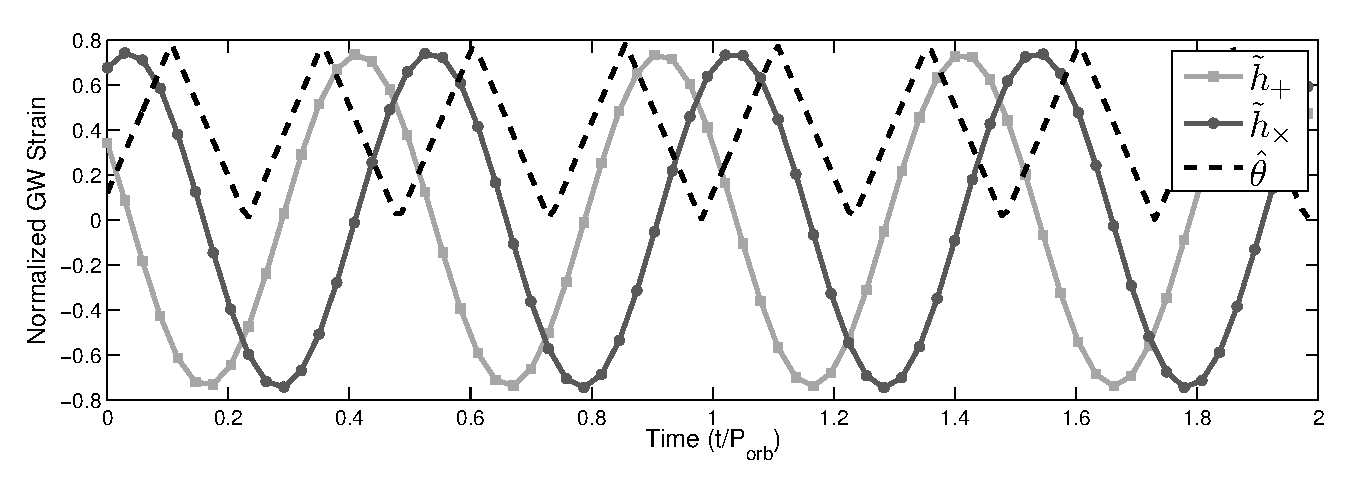
\includegraphics[width=\textwidth]{./figs/GWphase.eps}
\caption{Gravitational wave signals $\tilde{h}_+$ and
$\tilde{h}_{\times}$, as well as the estimated phase value
$\hat{\theta}$. Note that there are four locations where $\hat{\theta}=0$ in each orbital period, 
indicating the quadrature and conjunction phases. \eric{Updated the language in this caption a bit, and redid the figure
 for better label size}}
\label{fig.GWphase}
\end{figure*}

\eric{Expand this explanation to stress how important this is. This is the key for the multi-messenger aspect of the method.}

The $h_+(t)$ and $h_\times(t)$ waveforms in Eq.\
\ref{eqn.wahlquistPolarization} represent the expected signals that
will be observable by a gravitational wave observatory.  These
expressions can be solved for $\theta$ to give an estimate of the
binary phase as a function of time:
\begin{equation} \label{eqn.phase_est}
   \hat{\theta}(t) = \dfrac{1}{2}\cos^{-1}\left (
   \dfrac{2\sqrt{\tilde{h}_+^2(t) + \tilde{h}_\times^2(t) -
   \cos^2(\iota)}}{\sin^2(\iota)}\right )
\end{equation}
where $\tilde{h}_+$ and $\tilde{h}_{\times}$ are the measured
waveform amplitudes scaled by $h_{o}$, e.g. $h_+ = h_{o}\tilde{h}_+$.

There is a four-fold degeneracy in Eq.\ \ref{eqn.phase_est} due
to the square root and inverse cosine. This results in four locations
where $\hat{\theta}=0$ during each binary orbit, corresponding to the
phases where the projected distances between the binary components are maximized or minimized i.e. the quadrature and conjunction phases. 
The model lightcurve uses a value of $\phi=25^{\circ}$, resulting in
gravitational wave signals and phase estimate as shown in Figure
\ref{fig.GWphase}.



% =================================================================
\section{Model Implementation and Demonstration}\label{sec.demon}
Our accretion disc radius estimation method is now described explicitly and applied to the AM CVn system.  Lightcurve data from our model and the actual observed lightcurve \citet{1998ApJ...493L.105H} are both used to demonstrate the method.
Gravitational waveforms and model lightcurves are generated
using the model parameters in Section \ref{sec.modelParameters}.
Since gravitational wave observations do not yet exist for this
system, we regard this as a test of the method with partially real
data.

We assume that fundamental parameters of the system can be extracted,
i.e. component masses, secondary temperature, orbital period,
inclination, and luminosity distance, from which a stream overflow
model and lightcurve model for the ellipsoidal variations (EV) can
be generated. We also assume that the gravitational wave signals
$h_+(t)$ and $h_\times(t)$ have been disentangled and are separately
available. There will be a substantive number of multi-messenger 
binaries that can be simultaneously observed in EM and GW spectrums 
\citep{LLCN2013}; the gravitational wave data will provide accurate 
values for the component masses, the orbital period, and the 
inclination, all of which will inform the modeling described here.
\eric{This paragraph may be the right place to add in a note about the uncertainty in parameters, notably
the individual component masses. We should also acknowledge that while we are using ideal GW waveforms (which I noted that
we assume are separated by polarization), there will be some amount of noise with real observations. Just make a note of it and
move on.}

The method proceeds as follows:
\begin{itemize}
   \item Model accretion stream
   
   \item Model ellipsoidal variations
   
   \item Use GW signal to calibrate lightcurve to orbital phase
   
   \item Subtract EV from observational data -- remaining modulation
   should be due to hot-spot
   
   \item Determine phase offset between binary axis and hot-spot
   
   \item Use stream overflow model to determine radius of disc
\end{itemize}


\subsection{System Modeling}
The methods outlined in Section \ref{sec:geomFlux} have been used to model the
AM CVn lightcurve, which is shown against the observed lightcurve in
Figure \ref{fig.LC_output}.  Using our model parameters, the
calculated magnitude for this simulation is $m_{\text{sim}} \approx
14.18$, which matches the accepted value for AM CVn.  

The model output shown in figure \ref{fig.LC_output} displays the residuals between the observed data and the model fit in the bottom panel. The model performs reasonably well in recreating the qualitative features of the observed data given its simplicity, though it greatly overestimates the amount of dimming that occurs during the quadrature phases. These errors are likely due to omitting physical effects such as reflectance and limb darkening that would have small but noticeable effects on the total flux output. 

Our lightcurve model is used in two ways. First we assume that the model lightcurve generated by simulating the full AM CVn system is the observed lightcurve and proceed with the method from there, showing that the method can recover the disc radius well for the simulated data. In parallel we work with the \textit{true} lightcurve data where the full system model is not used. For each case a model of the EVs are required to perform the subtraction which results in the hot spot modulation, and so each demonstration utilizes the EV model generated by our simulation. Given the simple and predictable nature of EVs, this is a reasonable course of action.


%\note{eric: the obvious question anyone will ask is what do the residuals of that fit look like.  This is the obvious place to plot the residuals of DATA - SIMULATION, and talk generally about the discrepancies that are seen; the discrepancies are the things that will limit the method.  Don't shy away from the discrepancies --- note what they are, comment onwhether or not they will affect the demonstration here, and speculate on improvements that could address them.}

\subsection{EV Subtraction}

In order to locate the hot spot phase, the contribution to the 
lightcurve from the EV must be modeled and removed. The 
resulting EV from our model using the AM CVn parameters from table \ref{table.params} is shown in Figure \ref{fig.EV}.

\begin{figure}[h!]
\centering
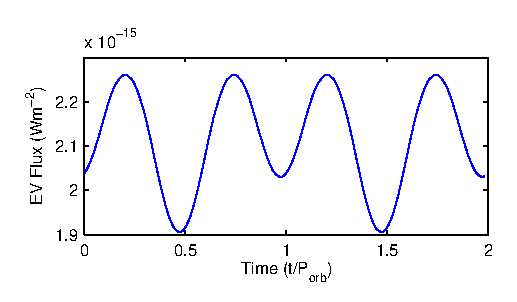
\includegraphics[width=\columnwidth]{./figs/EV.eps}
\caption{Ellipsoidal variation model output for Am CVn. This curve will be subtracted from
observed lightcurve to find the HS modulation after the correct initial phase $\theta_0$ is found.}
\label{fig.EV}
\end{figure}


In section \ref{sec.GWcal} the method for identifying the quadrature and conjunction phases using the gravitational wave signals was described. To compute the hot spot phase offset from the binary axis, we need to identify the conjunction phase in which the secondary Roche lobe is closest to the observer, as  the hot spot flux should peak briefly before that time. It is the phase difference between the hot spot flux peak and the following conjunction phase that we interpret as the hot spot phase offset. Using the synthetic GW signals, a binary phase estimate $\hat{\theta}(\tilde{t})$ is generated and shown in
figure \ref{fig.GWphase}. The conjunction and quadrature phases are
identified as the points where $\hat{\theta}(\tilde{t}) = 0$ ($\tilde{t} \equiv t/P_{orb}$), and since our EV model treats a quadrature phase for $\theta=0$, the
initial phase $\theta_0$ for the EV model will take one of four values
\begin{equation}
   \theta_{0,i} = 2\pi(1-0.25i-\tilde{t}_0)
\end{equation}
where $i \in \lbrace 0,1,2,3 \rbrace$, and $\tilde{t}_0$ is the first location where
$\theta(\tilde{t})=0$.

 Based on the overflow trajectory simulations, we expect the
phase of the HS peak output to lead the appropriate conjunction
phase. We make the reasonable assumption that the peak in the lightcurve corresponds closely to the peak in received hot spot flux, and so we choose the valley in $\hat{\theta}$ just behind the lightcurve peak to be the appropriate conjunction phase, making the previous $\tilde{t}=0$ point the quadrature phase we want for the initial EV phase, i.e. the point near $\tilde{t}=0.75$ in our demonstration data.

With both the EV model and initial phase estimate in hand, the estimated hot
spot modulation can be found by performing the subtraction $HS = OD - EV$ (abbreviations from table \ref{table.abbrev}). If the correct initial phase was chosen, the remaining variation in the lightcurve should be due to either HS modulation or eclipses. The subtraction results are shown in figure \ref{fig.subt2} for both the full model simulation (solid red curve) and the actual observed data (blue dots). The top panel illustrates the result of choosing an incorrect $\tilde{t}_0$ as the initial phase for the EV model, while the bottom panel shows the result of choosing the correct initial phase as described previously. 

\begin{table}[h]
\caption{Lightcurve Abbreviations}
\centering
\begin{tabular}{l l}
\hline \hline
Abbreviation & Meaning\\
\hline
OD & Observed lightcurve data\\
HS & Hot spot modulation\\
EV & Ellipsoidal variations\\
\hline
\end{tabular}
\label{table.abbrev}
\end{table}

%Using these as initial phase values for the EV model, the subtraction results obtained by assigning the desired conjunction phase and the preceding quadrature phase to $\theta_0$ in the EV model are shown in figure ***** . 

%The EV lightcurve is subtracted from the observed lightcurve data (OD), with the results for the synthetic lightcurve shown in Figure \ref{fig.subt1}, and for the true observed data in Figure \ref{fig.subt2}. 


\begin{figure}[h!]
\centering
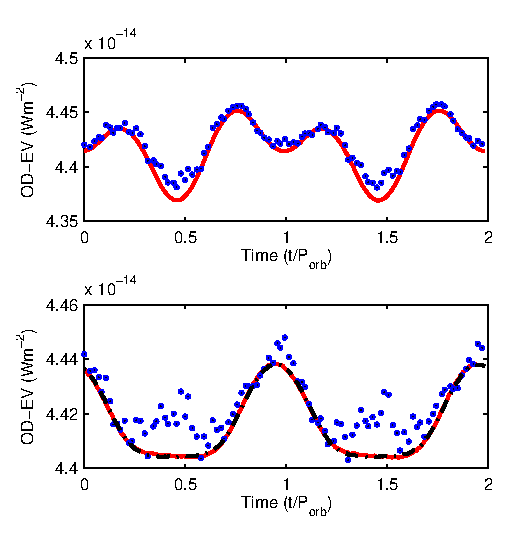
\includegraphics[width=\columnwidth]{./figs/AMCVnSubBoth.eps}
\caption{Results of the $HS = OD - EV$ subtraction for both the model data (red line) and observed data (blue dots) using the conjunction phase (incorrect) as $\theta_0$ (top panel) and the quadrature phase (correct) as $\theta_0$ (bottom panel). Also plotted in the bottom panel is the actual $HS$ output from the model (black dot-dash). The model subtraction result matches very closely to the model $HS$ output, but not perfectly due to errors discussed in the text.}
\label{fig.subt2}
\end{figure}





%\note{eric: note1 -- we should look at panels in fig 14 and decide how to reference them in the text.  Also, I think a red line version of Fig 13 overlaid on the resulting data subtraction in panel b of fig 14 may be useful}

%\note{eric: note2 -- the paragraph below introduces some numbers and 
%in particular makes some error estimates; this needs to be discussed 
%in context with the next section, which notes noisy data can be an 
%issue. What makes this confusing is I don't have any way of assessing 
%what these error estimates mean as compared to those you note before 
%using ``noise data''.}

\subsection{Disc Radius Estimate and Errors}

The subtraction $HS=OD-EV$ yields what should be the modulation in the
lightcurve due to the hot spot flux.  From here it is possible to
estimate the phase at which the hot spot flux peaks (the face-on view),
and therefore compute a value for the HS phase angle $\alpha_\star$.

Noise exists in both the simulated data and the observed data. In the simulated data this arises from the fact that the simulation samples are taken at a realistic rate (60 Hz), and numerical noise that is introduced by the finite discretization of the body surfaces. Due to the noise present in the lightcurves, we estimate the location of maximum HS flux output by fitting parabolas to random subsets of the lightcurve data surrounding the apparent peak in the $HS = OD - EV$ subtraction and taking the mean of the resulting parabola vertex locations as the orbital phase of the HS peak flux output $\theta_{HS}$. This process is illustrated in Figure \ref{fig.parabolas}. The HS phase offset $\phi_{HS}$ is then estimated by finding the phase difference between $\theta_{HS}$ and the conjunction phase following the initial phase, i.e. $\phi_{HS} = (\theta_0 + \pi/2) - \theta_{HS}$, and the corresponding disc radius is identified from the accretion stream simulations described in Section \ref{sec.Overflow}.

\begin{figure}[t]
\centering
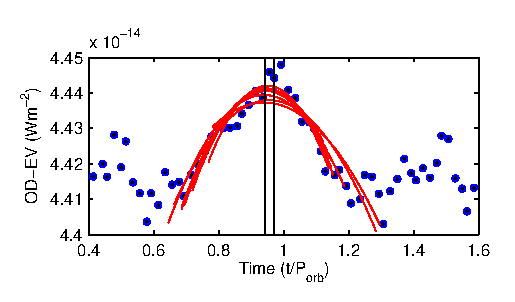
\includegraphics[width=\columnwidth]{./figs/AMCVn_parabolas.eps}
\caption{The parabola fitting procedure used to estimate the location of the observed HS peak output. Parabolas are fit to random subsets of the data surrounding the apparent peak near $ t=1 $. The average peak location (left hand black line) is found and regarded as the true peak location, $ \theta_{HS} $, which is then used to find the HS phase offset, $ \phi_{HS} $, relative to the subsequent conjunction phase (right hand black line).}
\label{fig.parabolas}
\end{figure}

For the model data using the random parabola procedure, we find a HS phase offset of $\phi_{HS} = 7.76^{\circ} \pm 1.6^{\circ}$. Using the overflow stream simulation, we find a corresponding disc radius estimate of $\hat{R}_D/a \approx 0.476 \pm 0.025$, where the error bars arise from various parabola fits. This gives an error for the mean value of $\approx 0.4 \%$ when compared with the accepted value of $0.478a$.

The noisy nature of the true observed data makes it less clear where the HS peak flux lies. We attempt the same fitting procedure and find HS phases in the approximate range $\phi_{HS} = 7.6^{\circ} \pm 2.8^{\circ}$. This translates to an estimated disc radius of $\hat{R}_D/a \approx 0.481 \pm 0.05$. With this method we find an estimation error of $\approx 0.6\%$.


%For the model data, we find the peak HS emission at time $\tilde{t}=0.9469$, and the
%corresponding conjunction phase at $\tilde{t}=0.9693$.  The angular
%difference between these points, and hence the HS phase, is
%\begin{equation}
%\phi_{HS} = (0.9693-0.9469)*360^{\circ} = 8.07^{\circ}
%\end{equation}
%Referring back to the accretion stream simulation displayed
%previously, this HS phase corresponds to a disc radius of $\hat{R}_D
%\approx 0.472a$. Comparing to the input disc radius $R_D = 0.478a$,
%this results in an estimation error of $\approx 1.3\%$. 

%The noisy nature of the true observed data makes it less clear
%where the HS peak flux lies. Two approaches are attempted here:
%to consider the largest valued data point after EV subtraction to be
%the HS peak, and to fit a parabola to some subset of the data
%surrounding the apparent peak. The first method results in a HS phase
%of $\phi_{HS} \approx -8.46^{\circ}$. This is a confusing result in
%that it suggests a hot spot that lags behind the conjunction phase,
%where we expect the HS peak to lead the conjunction phase in the
%lightcurve. 

%\note{eric: in the section above, the introduction of two letter 
%names to represent the different lightcurves is fine, but we probably 
%need to have some clear paragraph somewhere that introduces the 
%abbreviations.  Maybe a table that has in the first column the 
%abbreviation, and in the second column a brief description of what 
%lightcurve it is, together with a note as to whether it is observed 
%data, synthetic, or mock data (the GW are the only ones, in this case)}

% -------------------------------------------------
%\subsection{Ambiguity in noisy data}
%\note{eric: okay, i'm reading this now after the reorganization, and 
%I am not clear what this section is all about.  Did we do a new 
%simulation with extra noise added on top of it?}

%The accretion stream and ellipsoidal variation models are identical
%to those in the preceding sections. 



\section{Discussion}\label{sec.discussion}
The method described here is an independent method that is applicable
to mass-transferring galactic binaries observable by multi-messenger
campaigns involving gravitational wave and electromagnetic
observatories.  It is a method for measuring the accretion disk radius
in any compact binary system, \textit{whether it is eclipsing or not.}

Recent work has estimated that with even modest, sub-meter class 
telescopes, there will be hundreds of ultra-compact binaries that 
will be simultaneously detectable in gravitational waves and with EM 
telescopes \citep{LLCN2013}; thousands will be observable with 
multi-meter class telescopes, opening the potential to characterize 
the physical nature of an entire population of mass transferring 
binaries.

The model described here for measuring accretion disk radii assumes
the primary variation in the optical lightcurve can be identified
with a radiating hot spot on the disk, rotating about the primary with
the orbital frequency, $\omega_{o}$.  In low mass ratio systems like
AM CVn, it has been predicted that the accretion disk will suffer
tidal instabilities, deforming it into an eccentric precessing disk,
resulting in the phase offset angle varying in time, $\alpha_\star =
\alpha_\star(t)$.  This instability was first recognized in SU UMa stars,
and is thought to be responsible for the ``superhump'' phenomena in
the optical signature of CV stars.  The lightcurve of AM CVn is known
to exhibit a superhump signature, which could complicate the
measurement of the optical phase if it were not well characterized,
especially when tracked over long time periods.

The superhump mechanism has been well studied, and there is a known 
relationship between the periods of the binary orbit ($\tau_{o}$), the 
precessional period of the accretion disk ($\tau_{aa}$, period of 
apsidal advance), and the superhump signature ($\tau_{sh}$) given by
\begin{equation}
    \tau_{o}^{-1} =  \tau_{sh}^{-1} +  \tau_{aa}^{-1} \ .
    \label{PeriodTheory}
\end{equation}
For AM CVn, all three periods have been measured ($\tau_{o} = 1028.77$
s, $\tau_{sh} = 1051.2$ s, and $\tau_{aa} = 13.38$ hr; \citep{PHS},
\citep{1998ApJ...493L.105H}).  This allows the lightcurve to be
reduced and a measurement of the accretion disk made using the
difference in phase with a gravitational wave signal.  In principle,
the presence of the superhump signature, together with the disk radius
measurements described here, could be used in concert with
gravitational wave observations to measure the ellipticity of the
accretion disk.  This in turn can provide a method to probe
theoretical models of the pressure profile of the accretion disk 
\citep{2006MNRAS.368.1123G}.  This will be the focus of a future 
paper.

The analysis presented here also depends crucially on knowledge of the
trajectory of the matter stream which overflows from the secondary
Roche lobe into the sphere of influence of the white dwarf.  If the
hydrodynamic simulations of the overflow present an accurate picture
of the trajectory, then gravitational wave observations can provide a
new tool for probing the physical character of astrophysical systems.

\acknowledgments The author wishes to thank M.\ B.\ Larson for helpful
discussions and suggestions during the course of this work, and the 
late W.\ A.\ Hiscock for first suggesting the possibility of comparing 
phase measurements to probe ultra-compact binaries.  This work was 
supported by NASA award NNX13AM10G.

\bibliography{masterRefs}


\end{document}



%% ===================================================================
%% ===================================================================
%% ======== TIDBITS NOT TO LOSE ======================================
%% ===================================================================
%% ===================================================================
\begin{enumerate}
    \item [$\blacktriangleright$] A simple, parameterized model of the
    matter overflow stream will be constructed in the restricted three
    body approximation, providing a trajectory model of flow through
    the inner Lagrange point and along its inspiral toward the
    accretor in the binary.  This simulation work is currently being
    carried out by the PI's undergraduate student (Jake Knight, USU
    Physics) as part of his senior research project, and is similar in
    scope to early demonstrations in the literature
    \citep{Flannery1975}.  Early successful flow calculations are 
    shown in panel (B) of Figure \ref{fig.overflow}.
    
    \item [$\blacktriangleright$] The binary system parameters from
    mass transferring binaries in the LISA resolvable binaries will
    be used to seed the overflow code.  For the purposes of this
    study, only those binaries that are proximate enough to Earth to
    detect electromagnetically will be selected from the resolvable 
    binaries in our synthesis galaxies.
    
    \item [$\blacktriangleright$] The overall accuracy of the method
    is a function of the accuracy of the phase measurements, which
    depend on the electromagnetic luminosity and gravitational wave
    luminosity of the system.  The relative error between the two
    measurements constrain our ability to measure the offset phase
    angle $\alpha$.  The electromagnetic luminosity will be modeled
    from the impact of the overflow stream on the disk; the
    gravitational wave luminosity will be modeled from the resolvable
    binary parameters.
\end{enumerate}



A detailed theoretical model of AM CVn has been worked out, describing 
a variety of signals which are present in the photometric data 
\cite{Faulkner1972,Patterson1992, Patterson1993}.  This model suggests 
that AM CVn is a member of a class of variable stars which have 
periodic features in the lightcurve known as ``superhumps'' 
\cite{Vogt1982,Whitehurst88}.  The superhump mechanism proposes the 
existence of an eccentric precessing accretion disk, with a precession 
period which is slightly longer than the orbital period of the 
binary.  Knowing the superhump period, $P_{sh}$, and the precessional 
period of the accretion disk (apsidal advance), $P_{aa}$, one may 
predict the {\it orbital} period as
\begin{equation}
    P_{orb}^{-1} =  P_{sh}^{-1} +  P_{aa}^{-1} \ .
    \label{PeriodTheory}
\end{equation}
Photometry of AM CVn shows the existence of a superhump signature at 
$P_{sh} = 1051.2$ s, and the period of the accretion disk precession 
at $P_{aa} = 13.38$ hr.  Using Eq.\ (\ref{PeriodTheory}) this model 
has been used to predict a binary orbital period of $P_{orb} = 1028.77 
\pm 0.18$ s for AM CVn \cite{Patterson1993}.  Photometric observations 
by the CBA\footnote{The Center for Backyard Astrophysics (CBA) is a 
network of amateur astronomers (equipped with CCD photometry 
equipment) who monitor variable stars.  The network is managed by 
professional astronomers at Columbia University.} have recently 
confirmed an orbital period of $P_{orb} = 1028.7325 \pm 0.0004$ s 
\cite{1998ApJ...493L.105H}.


\bibitem[Hellings 1999]{HellingsPrivate} Hellings, R.\ W., private 
communication.

\bibitem[U. S. Standard Atmosphere 1976]{NationalAtmosphereModel} {\it 
U. S. Standard Atmosphere}, 1976, U.\ S.\ Government Printing Office, 
Washington, D. C.

\bibitem[Whitehurst 1988]{Whitehurst88} Whitehurst, R., 1988, Mon.\ 
Not.\ R.\ Astr.\ Soc.\, {\bf 232}, 35




%% ===================================================================
%% ===================================================================
%% ======== Change Log ======================================
%% ===================================================================
%% ===================================================================


4/8/2013: version - accretion03: Eric Addison
	- A bit more work in lightcurve simulation and demonstration section.

4/3/2013: version - accretion02: Eric Addison
	- Worked on implementation section a little
	- Changed over to bibtex instead of \bibitem style.
	- changed all \cite's to \citep's (maybe some cleanup needed for extra parens)

3/29/2013: version - accretion02: Eric Addison
	Worked on equations, text, and figures in overflow simulation section.
	noticed possible issues with equation of motion as written, made changes but kept old values in red.


